\chapter{Answers}
\label{cp:answers}

\section{Question 1}

\begin{importantbox}
    Review and understand the connections and differences of Schlieren technique and shadowgraph technique.
\end{importantbox}

Both the Schlieren and shadowgraph technique are used to visualize flow patterns. While both methods use properties of light to show the flow of air that would be invisible to the naked eye, the shadowgraph technique shows light ray displacement whereas the Schlieren method shows the ray refraction angle. The Schlieren method also displays a focused image using a knife edge to deflect light rays while the shadowgraph technique displays a shadow. Mathematically, the Schlieren method is related to the first derivative of the index of refraction whereas the shadowgraph method is related to the second derivative \citep{lecture9}.

\autoref{fig:schlieren_setup} shows the experimental setup of the Schlieren method and \autoref{fig:shadowgraph_setup} shows the experimental setup of the shadowgraph method. Note the absence of a knife edge in the shadowgraph method setup.

\begin{figure}[htpb]
    \centering
    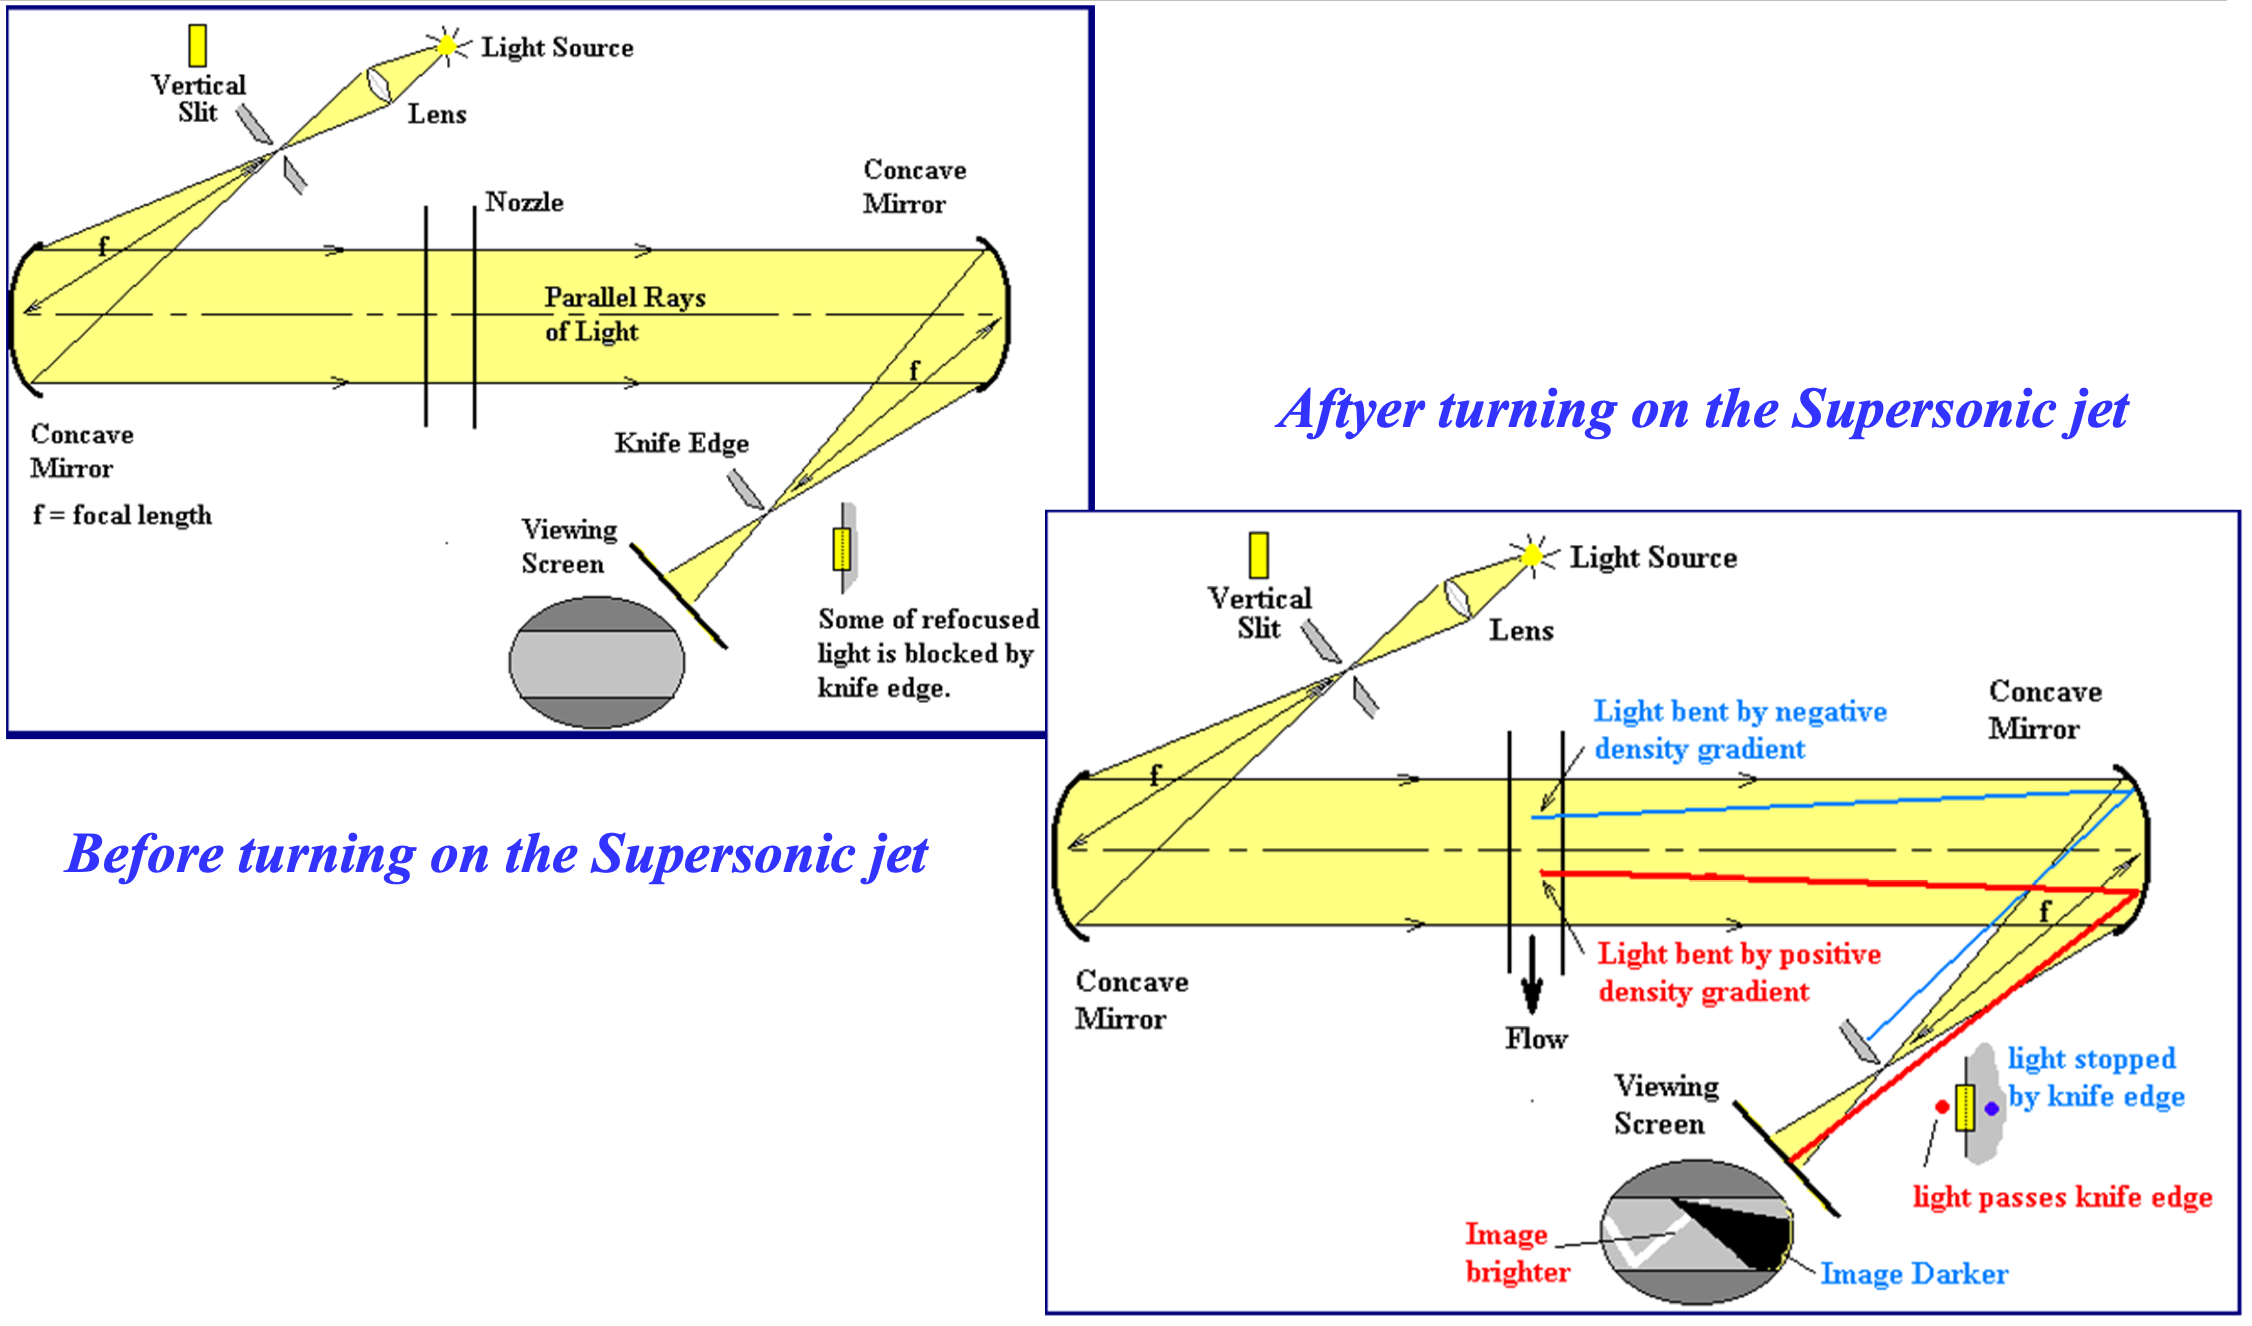
\includegraphics[width=\linewidth]{Figures/schlieren.png}
    \caption[Diagram of the Schlieren method.]{A diagram of the Schlieren method experimental setup \citep{lecture9}.}
    \label{fig:schlieren_setup}
\end{figure}

\begin{figure}[htpb]
    \centering
    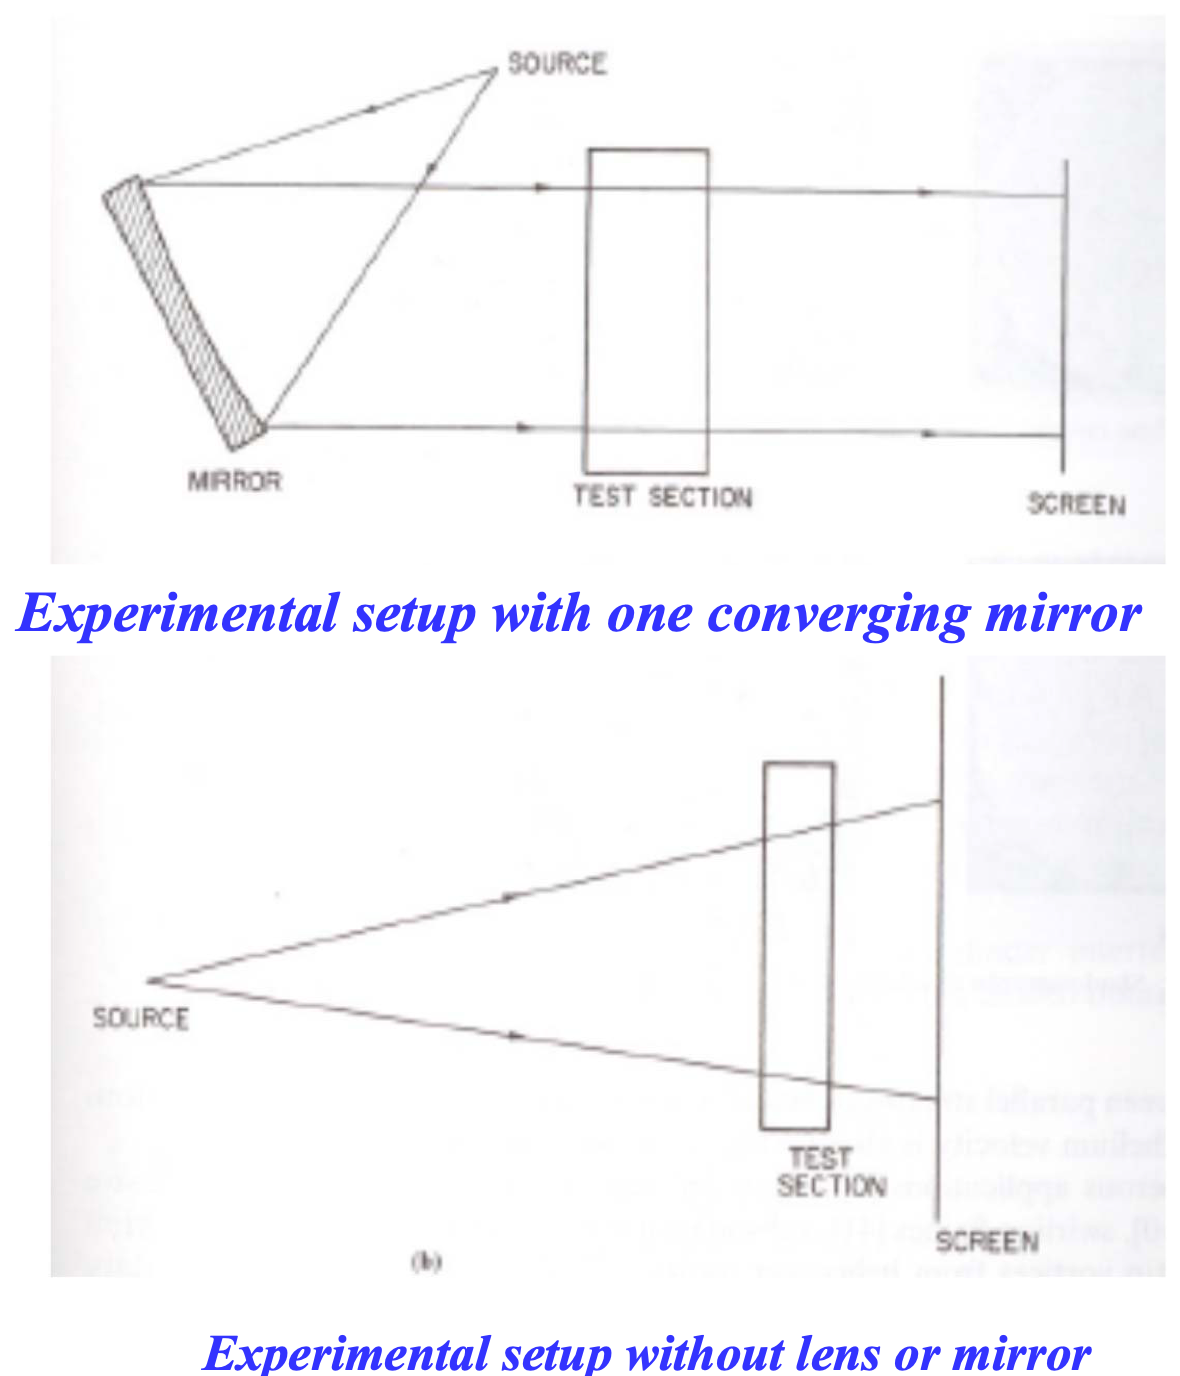
\includegraphics[width=0.8\linewidth]{Figures/shadowgraph.png}
    \caption[Diagram of the shadowgraph method.]{A diagram of the shadowgraph method experimental setup \citep{lecture9}.}
    \label{fig:shadowgraph_setup}
\end{figure}